\chapter{Evaluation}

\section{Performance compared to Gillian monoliths}

We first measure the performance of the stacks created using state model transformers against the performance of the original Gillian state models, that are built as large monoliths.

The evaluation is focused on testing the performance of state models across all modes supported by Gillian: Whole Program Symbolic Testing (WPST), OX Verification and UX Bi-Abduction. The files tested are either small tests used to test the engine, or larger verification targets extracted from real world code. Furthermore, when possible, the tests are also run with different optimisations of $\PMap$: $\ALocPMap$ and $\SplitPMap$.

All test logs were verified, to ensure full parity between all versions: the instantiations built using state model transformers yield the same results as the original instantiations. All passing tests pass, and all failing tests fail for the same reasons.

All tests were run on a 2020 MacBook Pro, with an M1 processor and 8GB of memory.

This evaluation will be split among the three different stacks originally supported by Gillian. As this evaluation concerns itself with performance only, we will not delve into the details of how these different languages work.
\begin{compactitem}
 \item WISL: a simple language, based on a linear heap, used to teach students. It supports WPST, verification and bi-abduction. Its state model can be constructed trivially, with the stack:
	\begin{align*}
 	 	\PMap(\Loc, \Freeable(\List(\Ex(\Val))))
	\end{align*}
 \item JavaScript: taking inspiration from JaVerT \cite{javert1, javert2}, Gillian comes with an instantiation for ES5 JavaScript. It supports WPST and verification -- bi-abduction ceased working due to changes during past developments, but could be fixed. It also comes with a WPST test suite to verify the Buckets-JS library. Its state can be modelled as:
	\begin{align*}
		\PMap(\Loc, \DynPMap(\Str, \Ex(\Val)) \bowtie \Ag(\Loc))
	\end{align*}
\item C: the third and last instantiation of Gillian supports a subset of C, using the CompCert-C verified compiler as an intermediary compilation step. It supports WPST, verification and bi-abduction. It comes with a WPST test suite to verify the Collections-C library, as well as a verification test suite for the AWS-Encryption-SDK library. Its state model is built as:
	\begin{align*}
		\PMap(\Loc, \Freeable(\BlockTree)) \bowtie \CGEnv
	\end{align*}
 \end{compactitem}

 \note{Add links / citations to Buckets-JS, Collections-C, CompCert-C, AWS-Encryption-SDK.}

\subsection{WISL}

\note{To do}

\subsection{JavaScript}

Originally the JavaScript instantiation of Gillian, Gillian-JS, was ported from JaVerT \cite{javert1,javert2}. We can reconstruct it as $\PMap(\Loc, \DynPMap(\Str, \Ex(\Val)) \bowtie \Ag(\Loc))$. Dissecting this construction, we first have $\DynPMap(\Str, \Ex(\Val))$, representing an object in JavaScript: a map from keys to values. On the other side of the partial product we have $\Ag(\Loc)$, corresponding to the location of the metadata of the object, in the same map. This allows to save some memory, as multiple objects can share metadata.

It comes with a few optimisations, to improve performance. Firstly, it splits the first level $\PMap$ entries between concrete and symbolic \emph{values}, avoiding substitutions in the concrete part. Secondly, it uses the abstract location mechanism mentioned previously, to index all entries by strings rather than expressions. Finally, it uses the OCaml \code{Hashtbl} module, a mutable data structure, rather than the immutable \code{Map} module -- this could improve performance, by avoiding creating copies of the map on modification. All of these optimisations are important, as the state in JavaScript code tends to be significantly large, with the first $\PMap$ regularly reaching 200 to 600 entries when running real life code (Buckets-JS, in this case) -- the highest recorded map size reaching 1179 entries for the \code{set3.gil} file.

Because the splitting between concrete and symbolic entries only occurs on the values of the first map, we can broadly replicate it by applying the split optimisation to the second map instead. To test all combinations of optimisations, we thus get the four following transformer stacks:
\begin{align}
\tag{TR}           & \PMap(\Loc, \DynPMap(\Str, \Ex(\Val)) \bowtie \Ag(\Loc)) \\
\tag{TR-ALoc}      & \ALocPMap(\DynPMap(\Str, \Ex(\Val)) \bowtie \Ag(\Loc)) \\
\tag{TR-Split}     & \PMap(\Loc, \SplitDynPMap(\Str, \Ex(\Val)) \bowtie \Ag(\Loc)) \\
\tag{TR-ALocSplit} & \ALocPMap(\SplitDynPMap(\Str, \Ex(\Val)) \bowtie \Ag(\Loc))
 \end{align}

The last version, TR-ALocSplit, is the closest in terms of applied optimisations to what Gillian-JS does. We note that the optimisation that uses \code{Hashtbl} is not applied to transformers, as they all use immutable data structures. While this has not been measured, it doesn't seem to have a significant performance impact. The opposite may be true, as while benchmarking we note that some time is spent copying the state in Gillian-JS; with transformers, a copy is instant.

This benchmark is split into three parts: WPST, verification, and Buckets (in WPST mode), each made up of respectively 21, 6 and 78 files. All tests were then run 30 times, for each state transformer stack and for Gillian-JS (labelled ``base''). The results can be seen in \autoref{fig:js-perf-bars}. The first insight this give us is that transformers seem to overall outperform the monolithic Gillian-JS, with an improvement ranging from 1.8 to 7.1\%. Another observation is that while both optimisations (ALoc and Split) seem to improve performance on the base instantiation, this improvement is dependent on what is the mode of execution, with ALoc being faster for verification, and Split being faster for WPST and Buckets (which is also WPST). This makes sense, as the split optimisation is only useful if there is a significant amount of concrete entries in the map, which there ought to be in whole program symbolic testing. We also note that the combination of the ALoc and Split optimisations seem to \emph{decrease performance} compared to when used separately or not used at all. This would indicate that the cost of both optimisations (abstract location translating, and checking for concreteness, respectively) becomes too much compared to the benefits.

\begin{figure}
	\centering
	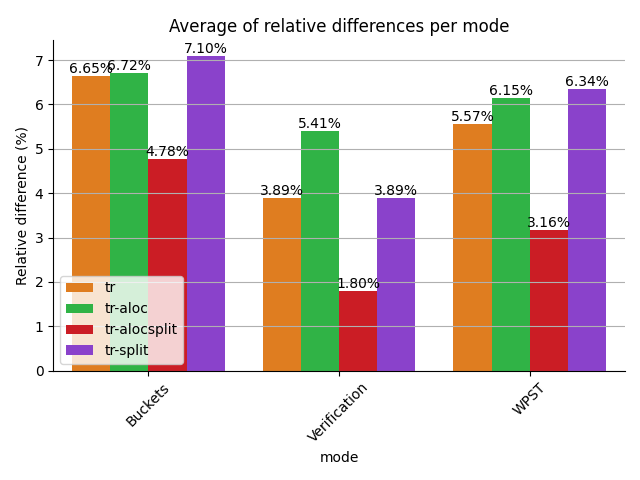
\includegraphics[width=10cm]{figures/js-perf-bars.png}
	\caption{Average of the relative difference in execution time for different test suites, per transformer stack}
	\label{fig:js-perf-bars}
\end{figure}

The initial conclusion we can reach from this is that transformer stacks are overall more performing than the monolithic alternative. One could of course imagine that a hyper-optimised monolith could be made with optimisations specific to the state model, which would then out-perform the more generic transformers. However in practice the size of such monoliths makes these optimisations hard to do, as code becomes complex quickly and makes changes harder -- in contrast, transformers are very simple to optimise, as they maintain a more generic structure. They are also easier to prove to be sound, as proofs can be done on the smaller elements rather than on the full state model.

Another idea this experiment seems to confirm is that the improvement given by optimisations is highly dependent on the context in which the engine is used, as simply switching between OX and WPST means one optimisation is better than the other. Transformers thus allow users to tailor the optimisations they use in their stack according to what code is verified, and how, by empirically measuring the performance of different alternatives (which are trivial to construct).

We may also take a closer look at how this time is spent within the engine. This is done by measuring the time before and after the entry point of each exposed method of the memory model, and summing the time spent within it. By looking at the average time per function call in the Buckets test suite (see \autoref{fig:js-avgtime-buckets}), we note that most memory actions (prefixed with ``ea/'', shorthand for \execac) are faster than in the base instantiation. Furthermore, and as mentioned previously, copying is orders of magnitude faster with transformers, since no work needs to be done.

\begin{figure}
	\centering
	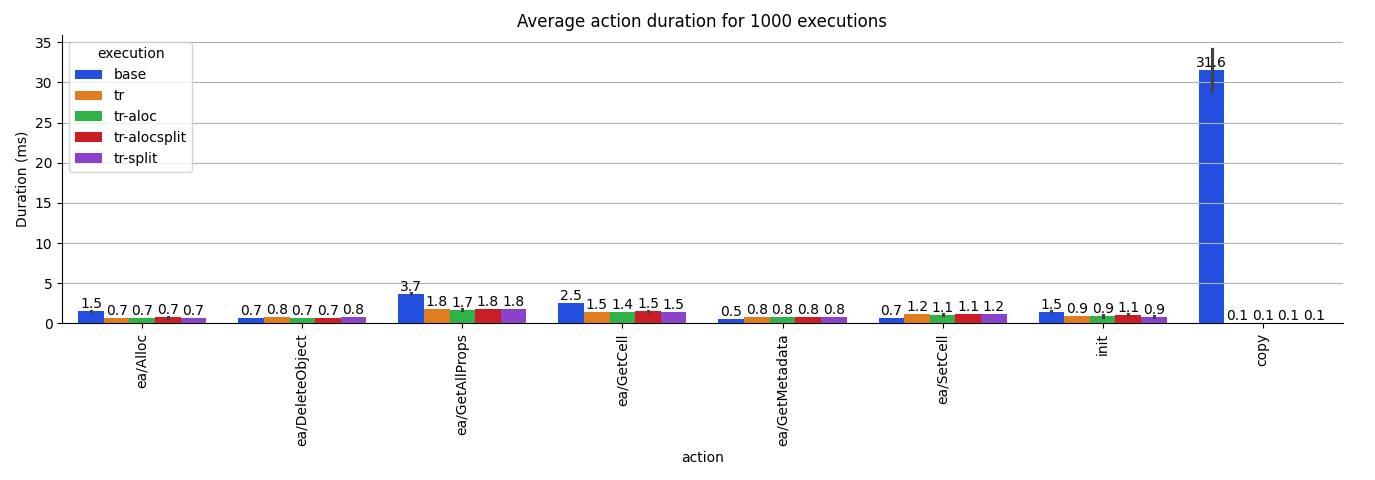
\includegraphics[width=\textwidth]{figures/js-avgtime-buckets.png}
	\caption{Average time spent per 1000 function calls in the Buckets test suite}
	\label{fig:js-avgtime-buckets}
\end{figure}

Looking at the average total duration for an execution of the test suite however (see \autoref{fig:js-timespent-buckets}), we note that the time taken by copying the state is minimal, as seen by the size of the ``other'' category. Instead, most time is spent during the \load{} (\code{GetCell}) action, which is called 11400 times (more than twice as many times as \store{}). The most notable improvement from the transformer construction is the reduction of the time spent getting a cell, reducing total time spent by 43\% (from 28.55 to 16.18ms). Because \load{} dominates the amount of action calls (see \autoref{fig:js-callcount-buckets}), this is sufficient to make up for the performance loss in \store{} and ``\code{GetMetada}'' (\load{} on the right side of the product).

\begin{figure}
	\centering
	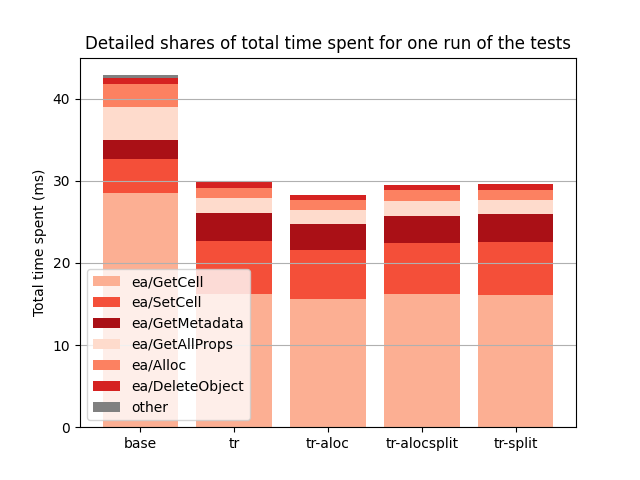
\includegraphics[width=10cm]{figures/js-timespent-buckets.png}
	\caption{Average total time spent per function in an execution of the Buckets test suite}
	\label{fig:js-timespent-buckets}
\end{figure}

\begin{figure}
	\centering
	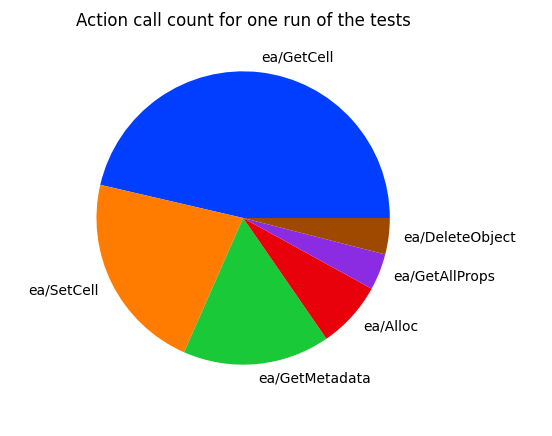
\includegraphics[width=8cm]{figures/js-callcount-buckets.png}
	\caption{Share of function calls for one execution of the Buckets test suite}
	\label{fig:js-callcount-buckets}
\end{figure}

If, instead of focusing on WPST with the Buckets code we focus on verification, the painted picture is significantly different. Indeed, while in WPST the memory model is only used for memory actions (as only the core engine is used), verification exercises the memory model quite differently, notably with \produce{} and \consume{}.

Most notably, this shows us that one of the leading differences in total time between different transformer instantiations is substitutions: TR-ALoc and TR-ALocSplit spending more than half as much time during substitutions than TR and TR-Split. This can be explained by the fact that with the ALoc optimisation, substitutions for the keys (abstract locations) can be filtered, meaning that if there is no substitution concerning abstract locations, we can simply map the values of the map without concerning ourselves with key conflicts. Without this, substitutions need to be applied to both key and value, and then all resulting keys need to be compared (an expensive process) to compose clashing entries. 

While this hasn't been measured, it is possible that the reason for the difference between time spent in substitutions between Gillian-JS and the transformer stacks is caused by the immutable data structures. With immutable data structures, copies of the full state are made for each substitution, which could be costly.

\begin{figure}
	\centering
	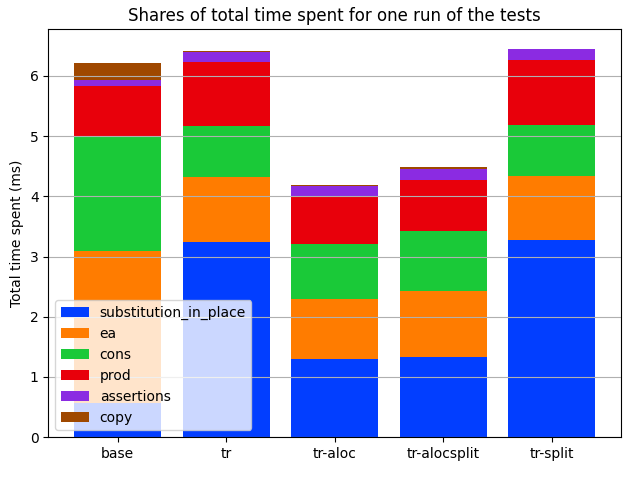
\includegraphics[width=10cm]{figures/js-timespent-verif.png}
	\caption{Share of grouped function calls for for one execution of the verification test suite}
	\label{fig:js-timespent-verif}
\end{figure}

Substitutions aside, we note how significantly less time is spent in \execac{} and \consume{} calls compared to the base state model; about 58\% and 55\% respectively. Again, this seems to indicate that simpler transformers tend to be more efficient than large monoliths.

Finally, we may compare development effort between the two state models. While not a perfect measure of complexity, lines of code (LOCs) are used, to compare the amount of code needed to instantiate each state model to get equivalent results. We only measure the lines of code in implementation files (\code{.ml}), ignoring interface files (\code{.mli}). We also ignore comments and whitespace lines. The results are shown in \autoref{fig:js-loc-count}. Here, we note that the amount of code needed tailored for each instantiation, seen in yellow (this includes constructing the stack, and applying necessary transformations, such as renaming actions and predicates, or adding a \code{delete} action) is minimal compared to Gillian-JS: only 246 LOCs. Most of the LOCs stem from the transformers code, which is shared and can be reused for different state models; a user of the engine would not need to worry about these. An engine developer is also likely to find it easier to work on the transformer code, as they are all independent from each other; unlike in the monolith where all elements have direct dependencies.

\begin{figure}
	\centering
	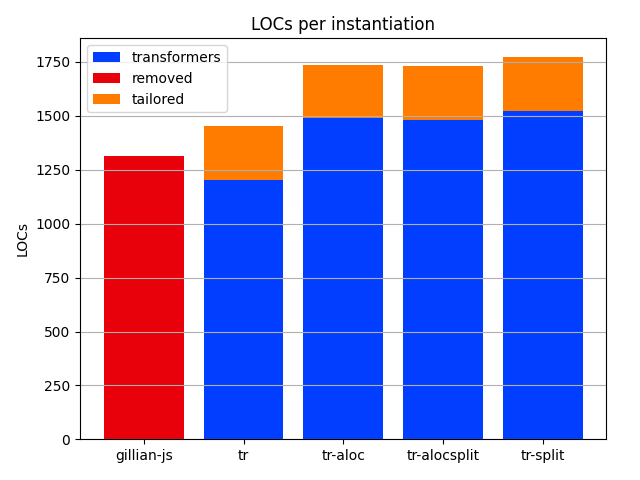
\includegraphics[width=10cm]{figures/js-loc-count.png}
	\caption{Number of lines of code per JS instantiation}
	\label{fig:js-loc-count}
\end{figure}

\subsection{C}

An instantiation of Gillian has been made for C, using the verified compiler CompCert-C \cite{gillian2}. It's memory model can be replicated as $\PMap(\Loc,\Freeable(\BlockTree)) \bowtie \CGEnv$. An important distinction from the JavaScript instantiation is that we can't replicate Gillian-C's behaviour only with the transformers introduced thus far. Indeed, C allows one to read parts of values (for instance, extracting two \code{int}s from a \code{long}), and Gillian-C also supports objects of symbolic size, which is not possible with $\List$ \note{why? Need to ask, I'm not sure}. Instead, we thus use the $\BlockTree$ state model, tailored for C, which supports the above uses. We will not go into details of how it works. Gillian-C also has a \emph{global environment} system, which allows storing pointers to function definitions in an agreement-like map: we import this system in $\CGEnv$.

As such, the Gillian instantiation for C using transformers uses a mix of generic transformers ($\PMap$, $\Freeable$) and of custom built state models ($\BlockTree$). The $\BlockTree$ code is mostly imported from Gillian-C, with minor modifications to match the structure of state models used for transformers. In comparison, the instantiation for JavaScript only uses generic transformers. This shows the flexibility of our approach, as it allows both for constructions that only rely on state model transformers, as well as hybrid constructions using specialised elements along with the generic ones.

In an effort to verify that the improvements from the optimised $\PMap$ versions are carried between languages, we also provide several C instantiations:
\begin{align}
\tag{TR}       & \PMap(\Loc, \Freeable(\BlockTree)) \bowtie \CGEnv \\
\tag{TR-ALoc}  & \ALocPMap(\Freeable(\BlockTree)) \bowtie \CGEnv \\
\tag{TR-Split} & \SplitPMap(\Loc, \Freeable(\BlockTree)) \bowtie \CGEnv
\end{align}

Gillian-C supports WPST, verification and bi-abduction with UX reasoning. It uses an abstract location optimisation, similarly to what was described previously, and immutable data structures (unlike Gillian-JS's use of \code{Hashtbl}).

This benchmark is split into five parts: WPST, verification, bi-abduction, Collections-C (in WPST mode) and AWS code (in verification mode), each made up of respectively 8, 6, 7, 159 and 10 files. All tests were run 50 times, except the AWS test suite that was executed 10 times\footnote{This is simply because verifying the AWS code takes \emph{significantly} longer than the rest.}.

The general results can be seen in \autoref{fig:c-perf-bars}. Here again, we note a significant performance improvement compared to the monoliths in Gillian-C, in particular for the AWS and bi-abduction suites. As for the optimisations, we get inconsistent results: they seem to improve performance for all modes but for AWS. 

An interesting observation is that transformers seem to still yield a better performance even when mixed with more complex state models, where most of the implementation still resides in large complex elements.

\begin{figure}
	\centering
	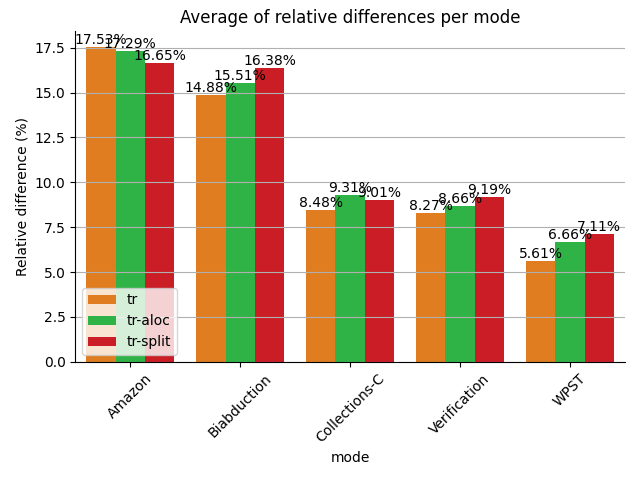
\includegraphics[width=10cm]{figures/c-perf-bars.png}
	\caption{Average of the relative difference in execution time for different test suites, per transformer stack}
	\label{fig:c-perf-bars}
\end{figure}

We may now look into the detailed rundown of the time spent; we will focus on Collections-C WPST and the AWS encryption SDK verification, as these correspond to real world code (whereas the other test suites only use simple data structures, and are primarily useful for ensuring parity).

When looking at the time spent in each function for each instantiation (see \autoref{fig:c-timespent-collectionsc}), the main takeaway is that two most common actions, $\code{mem\_store}$ and $\code{mem\_load}$, are both faster than the original version; about 20\% and 25\% respectively. This is significant, considering more than 75\% of memory actions in Collections-C is a load or a store.

\begin{figure}
	\centering
	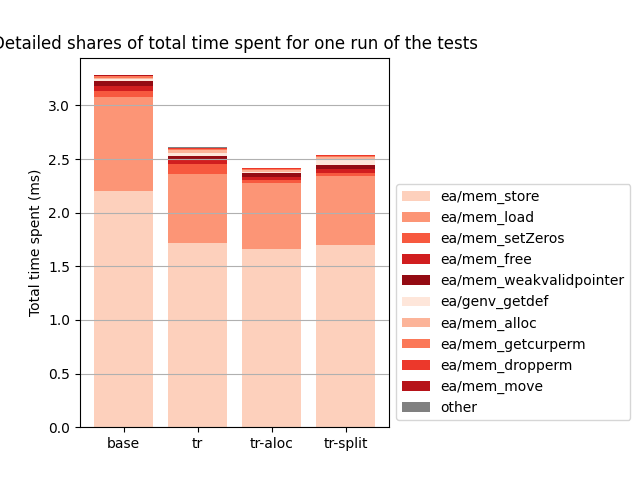
\includegraphics[width=10cm]{figures/c-timespent-collectionsc.png}
	\caption{Average total time spent per function in an execution of the Collections-C test suite}
	\label{fig:c-timespent-collectionsc}
\end{figure}

This story is however wildly different for AWS code, which uses verification rather than WPST. Here, memory actions only represent a fraction of the total time spent, which is instead dominated by mainly \consume, as well as \produce, as seen in \autoref{fig:c-timespent-aws}. Here we note slight improvements in time for most categories, again seeming to indicate that the more generic approach is generally more performant.

\begin{figure}
	\centering
	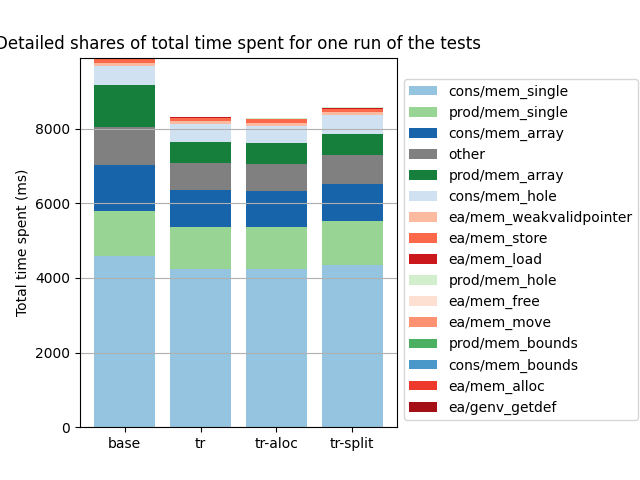
\includegraphics[width=10cm]{figures/c-timespent-aws.png}
	\caption{Average total time spent per function in an execution of the AWS header encryption SDK test suite}
	\label{fig:c-timespent-aws}
\end{figure}

Importantly, the charts for TR, TR-ALoc and TR-Split are extremely similar, for both Collections-C and AWS code; we can thurs hardly make a hypothesis as to which optimisation is better suited. This is in part due to the fact these optimisations excel in larger maps, as was the case for JavaScript. In C, maps are instead rather small; for Collections-C, the map size tends to fluctuate between 15 and 35 elements, with the maximum recorder reaching 52 elements. For AWS, its size is between 10 and 20 elements, maxing at 20. This in particular explains why the optimisations are detrimental for the AWS test suite: because the maps are always small, the cost of both optimisations regularly outweighs their improvement.

We now compare the complexity of instantiations, using LOCs. Here, we delve into more details on the reason for each line count. In particular, we see that the majority of the state model is the same; the modified part representing $\BlockTree$ and $\CGEnv$, which are lightly modified to fit into the transformers setup, while the untouched part represents the internal modules used by the C instantiations (for instance, to encode permissions, or memory chunks). Finally, the removed part of the code is trivially replaced with minimal constructions, using $\PMap$ and $\Freeable$. Some tailored code is also required, to ensure the construction matches the interface of Gillian-C. This again shows that even for more complex state models that require a significant amount of customised code, using transformers reduces the amount of code required exclusively for that instantiation -- since some can be in a shared transformers library -- while providing some performance gains for free.

\begin{figure}
	\centering
	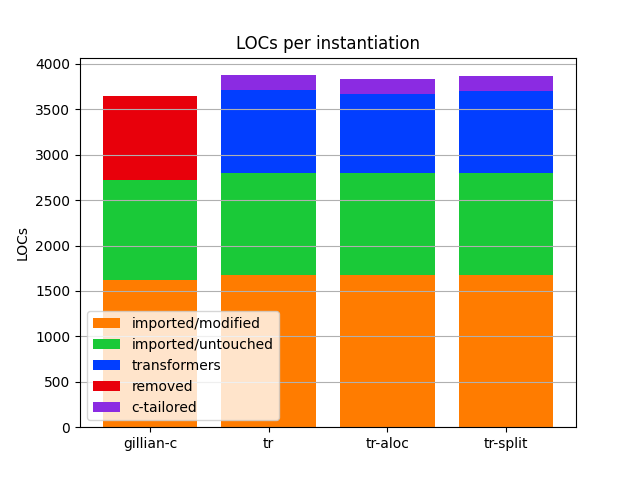
\includegraphics[width=10cm]{figures/c-loc-count.png}
	\caption{Number of lines of code per C instantiation}
	\label{fig:c-loc-count}
\end{figure}









